\chapter{Boson simulations}
\label{ch:Simulations}

\section{Introduction}
\label{sec:SimIntro}
This formed the bulk of the experimental work in my PhD. Roughly speaking, we
take a hamiltonian, \(\mat{H}\) and exponentiate it to get a load of unitaries
(\(\mat{U}=e^{-i\mat{H}t}\)) at a series of timesteps. Using a decomposition
similar to the one in \cite{reck} we can implement these on a single
circuit.

Two physical implementations: bulk optics and integrated optics. I was
responsible for the calibration of the bulk circuit (crapusoids), writing the
control code, and taking a large portion of the data. I trained DTC student
Chris Sparrow in the operation of the experiment.

\begin{figure}
  \centering
  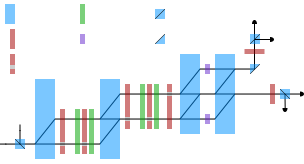
\includegraphics{figures/circuit.pdf}
  \caption[A schematic of the bulk optics circuit used for simulations.]
  {A schematic of the bulk optics circuit. Two photons are injected at
  the left of the circuit in orthogonal polarisations (\(\ket{H}\) indicates
  horizontal and \(\ket{V}\) indicates vertical), using an in-fibre polarising
  beamsplitter (PBS) to combine the two photons into a single path. The circuit
  operates in a combined path/polarisation encoding, where polarising beam
  displacers (PBD) are used to convert between the two. Operations are performed
  with fixed quarter waveplates (QWP) and polarisation flips (X), and variable
  angle half waveplates (HWP). After the operations are complete,
  polarisation-sensitive detection is performed using further PBS elements and
  single photon avalanche diodes. We label the detectors A through D.}
  \label{fig:circuit}
\end{figure}

\section{Quantized vibrational states}
\label{sec:Phonons}
More background: introduce the idea of quantized vibrational states and present
the data for the 4-atom ring. I took the data, and did some of the analysis.

\section{Molecular vibrations}
\label{sec:Molecules}
Simulating phonons in the harmonic limit corresponds to vibrations of molecules.

\section{PT-symmetric systems}
\label{sec:PT}
Taking a non-Hermitian hamiltonian, \(\mat{G}\) corresponds to an open system
with loss and/or gain. A system with balanced but spatially separated loss and
gain is \pt-symmetric. Exponentiating this hamiltonian gives us a non-unitary
time-evolution operator, \(\mat{V}\). Using unitary dilation, we implement this
as a sub-matrix of a unitary operator. Physically, this corresponds to coupling
the system to an environment with an equal number of spatial modes.
